\section{Hardware}

The hardware components of the system are minimal and were selected on cost and suitability. There are only two main hardware components in the system a Raspberry Pi 4 microcontroller and a Pi Cam. Otherwise there's only one other machine whose purpose is to house the database and run the user interface which could be performed by any moderately powerful machine with network capabilities.

\subsubsection{Node Hardware}

A microcontroller was required to perform the tasks of a node and the Raspberry Pi 4 was selected for its low cost, sufficiently powerful processor, small size, networking capability, operating system compatability, usb and Pi Cam compatability and its large online community. All of these factors made the Raspberry Pi an excellent choice for rapidly prototyping a computer vision system. The Pi Camera is a proprietary piece of camera hardware the integrates easily with the Raspberry Pi microcontroller and is similarly inexpensive, captures colour and a sufficient definition and frame rate. Figure \ref{fig:raspi_gear} shows the microcontroller with camera connected. Appendix [XXXXX] gives the full specifics of both of these pieces of hardware.

\begin{figure}[H]
    \centering
    \centering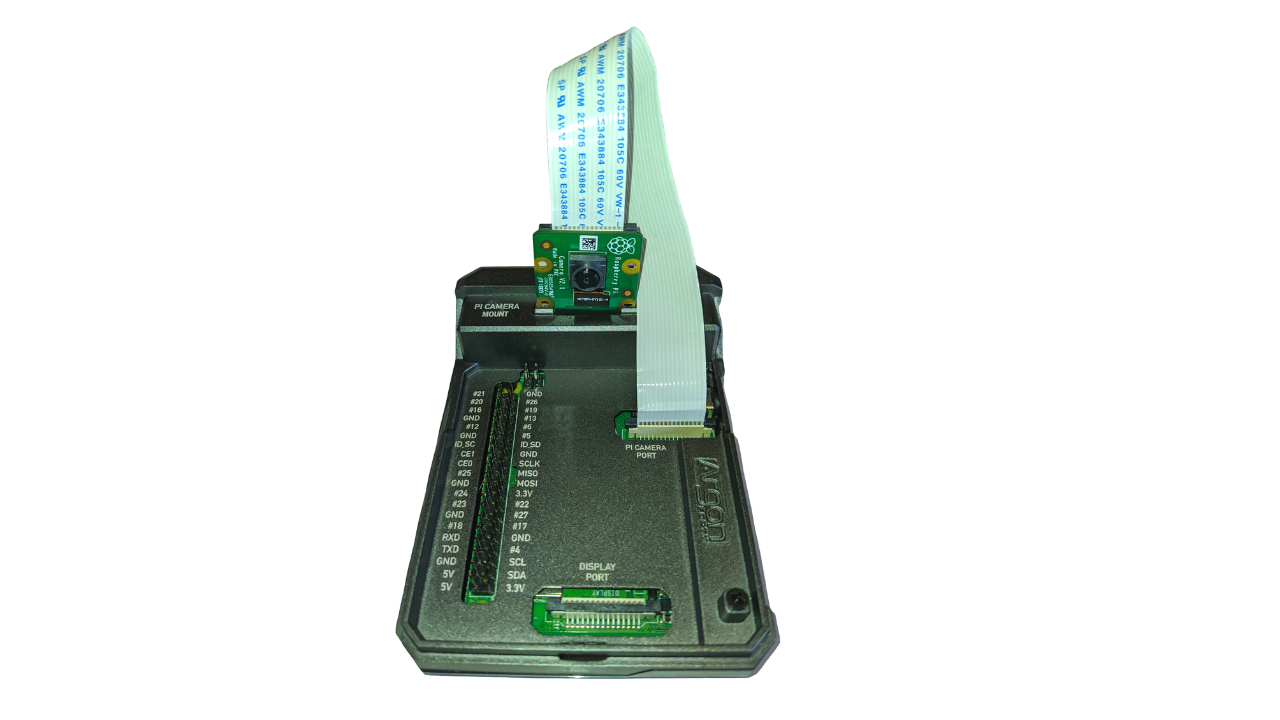
\includegraphics[width = 0.8\textwidth]{design/hardware/gear_improved}
    \caption{Raspberry Pi 4 and Pi Cam connected.}
    \label{fig:raspi_gear}
  \end{figure}
  